\documentclass{report}

\input{preamble}
\input{macros}
\input{letterfonts}

\usepackage{tikz}
\usepackage{tikz-3dplot}
\usepackage{amsmath}
\usepackage{amssymb}
\usepackage{pgfplots}
\usepackage{smartdiagram}
\usepackage{xcolor}
\usepackage{forest}
\usepackage{tikz-3dplot}
\usepgfplotslibrary{colormaps}
\usepgfplotslibrary{groupplots}
\pgfplotsset{compat=newest}

\usesmartdiagramlibrary{additions}

\title{\Huge{Temporary Doc}\\Calc 3}
\author{\huge{Giacomo Cappelletto}}
\date{23/10/24}

\begin{document}


\maketitle
\newpage
\pdfbookmark[section]{\contentsname}{toc}
\tableofcontents
\pagebreak

\chapter{Vector Valued Functions $f:\mathbb{R} \rightarrow \mathbb{R}^n$}

\ex{Problem with Multiple Surfaces}{
	The solid common to the cylinders bounded by \( z = \sin x \) and \( z = \sin y \) over the region
	\[
		R = \{ (x, y) : 0 \leq x \leq \pi, \; 0 \leq y \leq \pi \}.
	\]
	We define the domain \( D \) as
	\[
		D = \{ (x, y, z) : (x, y) \in R, \; 0 \leq z \leq \min(\sin x, \sin y) \}.
	\]

	To solve this problem, we will:

	\begin{enumerate}
		\item Consider one-fourth of the volume under the intersection of the two cylinders, taking advantage of symmetry.
		\item Identify the bounding conditions for \( z \) in each quadrant.
		\item Set up and compute the triple integral over \( D \) to find the volume.
	\end{enumerate}

	Given the symmetry, we restrict our analysis to the region
	\[
		0 \leq x \leq \frac{\pi}{2}, \quad 0 \leq y \leq \frac{\pi}{2}.
	\]
	In this quadrant, \( z \) is bounded by \( \min(\sin x, \sin y) \), which means \( z \leq \sin y \) in the region \( R_1 \), where \( \sin y \leq \sin x \).

	For region \( R_2 \) (where \( \sin x \leq \sin y \)), we have \( z \leq \sin x \). By observing symmetry, the volume in each quadrant contributes equally, so we can calculate the volume in this restricted region and multiply by 4.

	The bounds for \( x \) and \( y \) are:
	\[
		0 \leq y \leq \pi, \quad y \leq x \leq \pi - y.
	\]
	Thus, we set up the volume integral as follows:
	\[
		V = 4 \int_0^{\pi/2} \int_0^{\sin y} \int_y^{\pi - y} \, dx \, dy \, dz.
	\]

	Evaluating the integral:
	\[
		V = 4 \int_0^{\pi/2} \int_0^{\sin y} \left( \int_y^{\pi - y} dx \right) \, dy \, dz.
	\]

	Upon computation, this integral yields:
	\[
		V = \pi - 2.
	\]


	The key idea was to leverage the symmetry of the intersection region, focusing on one-fourth of the area and then scaling up by a factor of 4. By analyzing the geometry, we found that \( z \) was bounded by \( \sin y \) in region \( R_1 \). From there, the triple integral was computed over \( x \), \( y \), and \( z \) to yield the final volume of the region.
}

\begin{center}
	\begin{tikzpicture}
		\begin{axis}[
				width=12cm,
				height=12cm,
				view={60}{45},
				xlabel=$x$,
				ylabel=$y$,
				zlabel=$z$,
				xmin=0, xmax=3.1416,
				ymin=0, ymax=3.1416,
				zmin=0, zmax=1.2,
				grid=major,
				colormap/cool,
				xtick={0, 1.5708, 3.1416},
				xticklabels={$0$, $\frac{\pi}{2}$, $\pi$},
				ytick={0, 1.5708, 3.1416},
				yticklabels={$0$, $\frac{\pi}{2}$, $\pi$},
				samples=50,
				domain=0:3.1416,
				y domain=0:3.1416,
				trig format=rad,
			]

			% Surface for z = sin(x)
			\addplot3[
				surf,
				samples=50,
				domain=0:3.1416,
				y domain=0:3.1416,
				opacity=0.8,
			]
			{sin(x)};

			% Surface for z = sin(y)
			\addplot3[
				surf,
				samples=50,
				domain=0:3.1416,
				y domain=0:3.1416,
				opacity=0.8,
			]
			{sin(y)};

			% Boundary lines
			\addplot3[
				domain=0:3.1416,
				samples=50,
				thick,
				color=black,
			]
			({x},{0},{0});
			\addplot3[
				domain=0:3.1416,
				samples=50,
				thick,
				color=black,
			]
			({x},{3.1416},{0});
			\addplot3[
				domain=0:3.1416,
				samples=50,
				thick,
				color=black,
			]
			({0},{y},{0});
			\addplot3[
				domain=0:3.1416,
				samples=50,
				thick,
				color=black,
			]
			({3.1416},{y},{0});

			% Cross-section curves
			\addplot3[
				color=red,
				thick,
				domain=0:3.1416,
				samples=50,
			]
			({x},{1.5708},{sin(x)});

			\addplot3[
				color=blue,
				thick,
				domain=0:3.1416,
				samples=50,
			]
			({1.5708},{y},{sin(y)});

			% Height indicator lines
			\foreach \x in {0.5,1,1.5} {
					\addplot3[
						dashed,
						color=gray,
					] coordinates {
							(0,\x,0)
							(3.1416,\x,0)
						};
					\addplot3[
						dashed,
						color=gray,
					] coordinates {
							(\x,0,0)
							(\x,3.1416,0)
						};
				}

			% Add legend
			\addlegendentry{$z = \sin(x)$}
			\addlegendentry{$z = \sin(y)$}
			\addlegendentry{Boundaries}
			\addlegendentry{$x$-cross section}
			\addlegendentry{$y$-cross section}

		\end{axis}
	\end{tikzpicture}
\end{center}

\section{Polar Coordinate System}

\dfn{Polar Coordinates Overview}{
	The polar coordinate system is a two-dimensional coordinate system in which each point on a plane is determined by a distance from a reference point (often called the origin or pole) and an angle from a reference direction (usually the positive \( x \)-axis). The two coordinates are:

	\begin{itemize}
		\item \( r \): the radial distance from the origin to the point.
		\item \( \theta \): the angular coordinate, representing the angle in radians (or degrees) between the positive \( x \)-axis and the line connecting the origin to the point.
	\end{itemize}

	A point \( P \) in the plane can therefore be represented in polar coordinates as \( (r, \theta) \).
}

\dfn{Relationship Between Cartesian and Polar Coordinates}{
	In Cartesian coordinates, a point \( P \) can be represented as \( (x, y) \). We can convert between Cartesian and polar coordinates with the following relations:

	\begin{align*}
		x      & = r \cos \theta                   \\
		y      & = r \sin \theta                   \\
		r      & = \sqrt{x^2 + y^2}                \\
		\theta & = \arctan\left(\frac{y}{x}\right)
	\end{align*}

	These equations allow for the translation of a point's position between Cartesian and polar forms, showing the adaptability of the polar system for various types of analyses, especially when working with circular or rotational symmetry.
}

\begin{center}
    \begin{minipage}{0.45\textwidth}
        \centering
        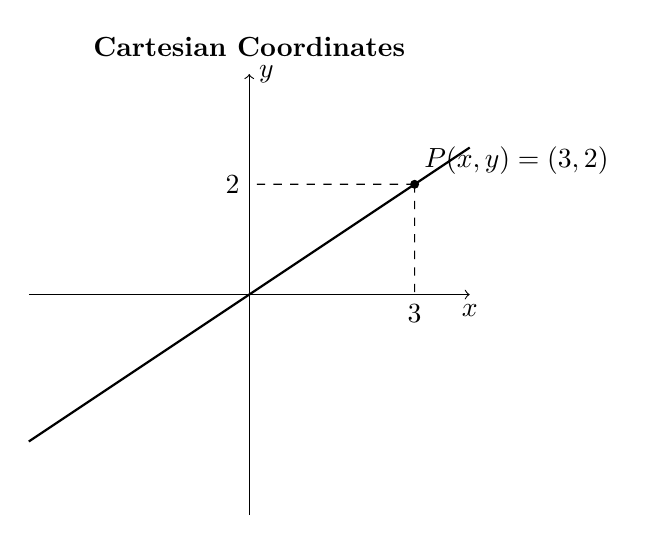
\begin{tikzpicture}[scale=0.7]
            % Cartesian coordinate system diagram
            \node at (0, 4.5) {\textbf{Cartesian Coordinates}};

            % Draw axes
            \draw[->] (-4, 0) -- (4, 0) node[anchor=north] {\( x \)};
            \draw[->] (0, -4) -- (0, 4) node[anchor=west] {\( y \)};

            % Draw point and line
            \coordinate (P) at (3,2); % Point P at (3,2)
            \draw[thick] (-4,-8/3) -- (4,8/3); % Line through origin and point (slope 2/3)

            % Mark point P
            \filldraw (P) circle (2pt) node[anchor=south west] {\( P(x, y) = (3, 2) \)};

            % Draw dashed lines to x and y axes for clarity
            \draw[dashed] (P) -- (3,0) node[anchor=north] {3};
            \draw[dashed] (P) -- (0,2) node[anchor=east] {2};
        \end{tikzpicture}
    \end{minipage}%
    \hspace{0.05\textwidth} % Space between the two diagrams
    \begin{minipage}{0.45\textwidth}
        \centering
        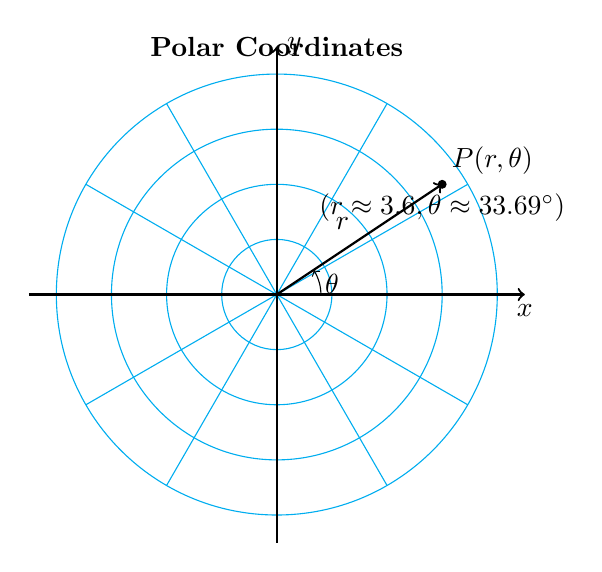
\begin{tikzpicture}[scale=0.7]
            % Polar coordinate system diagram
            \node at (0, 4.5) {\textbf{Polar Coordinates}};

            % Draw polar grid
            \foreach \r in {1, 2, 3, 4} {
                \draw[cyan, thin] (0,0) circle (\r);
            }
            \foreach \a in {0, 30, 60, 90, 120, 150, 180, 210, 240, 270, 300, 330} {
                \draw[cyan, thin] (0,0) -- (\a:4);
            }

            % Draw axis lines with labels
            \draw[->, thick] (-4.5,0) -- (4.5,0) node[anchor=north] {\( x \)};
            \draw[->, thick] (0,-4.5) -- (0,4.5) node[anchor=west] {\( y \)};

            % Draw point and radial line
            \coordinate (O) at (0,0);
            \coordinate (P) at (3,2); % Point P in polar coordinates (approx r=3.6, theta=33.69 degrees)
            \draw[->, thick] (O) -- (P) node[midway, anchor=south east] {\( r \)};
            \filldraw (P) circle (2pt) node[anchor=south west] {\( P(r, \theta) \)};

            % Draw angle arc
            \draw[->] (0.8,0) arc [start angle=0, end angle=33.69, radius=0.8];
            \node at (1,0.2) {\( \theta \)};

            % Label r and theta
            \node at (P) [anchor=north] {\( (r \approx 3.6, \theta \approx 33.69^\circ) \)};
        \end{tikzpicture}
    \end{minipage}
\end{center}

\begin{center}
	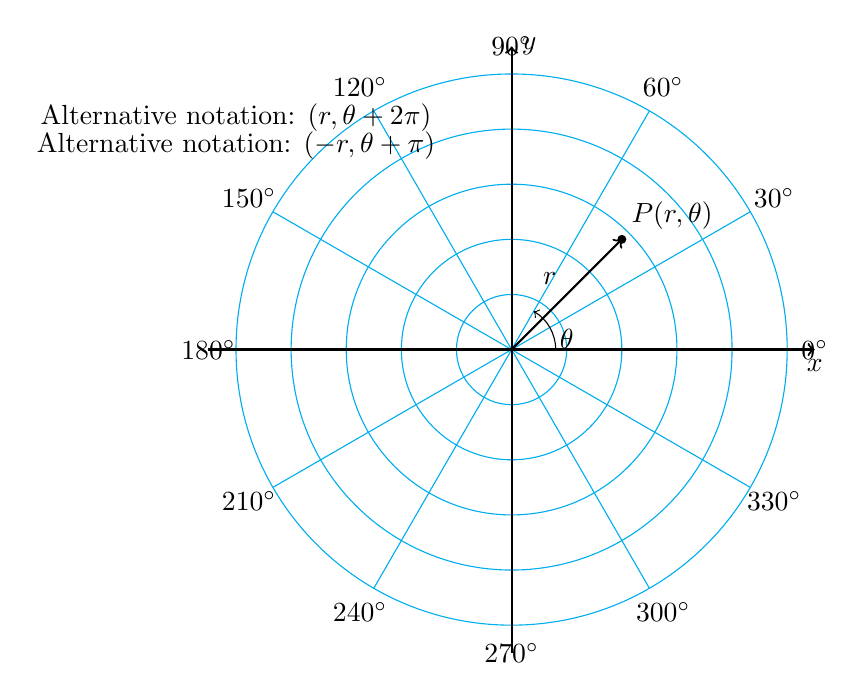
\begin{tikzpicture}[scale=0.7] % Adjust the scale here to resize the diagram
		% Draw concentric circles
		\foreach \r in {1, 2, 3, 4, 5} {
				\draw[cyan, thin] (0,0) circle (\r);
			}

		% Draw radial lines and angle labels
		\foreach \a in {0, 30, 60, 90, 120, 150, 180, 210, 240, 270, 300, 330} {
				\draw[cyan, thin] (0,0) -- (\a:5);
				\node at (\a:5.5) {\a$^\circ$};
			}

		% Draw axis lines with labels
		\draw[->, thick] (-5.5,0) -- (5.5,0) node[anchor=north] {\( x \)};
		\draw[->, thick] (0,-5.5) -- (0,5.5) node[anchor=west] {\( y \)};

		% Draw radial line for the point P
		\coordinate (O) at (0,0);
		\coordinate (P) at (2,2); % Set r=4 and angle=60 degrees
		\draw[->, thick] (O) -- (P) node[midway, anchor=south east] {\( r \)};
		\filldraw (P) circle (2pt) node[anchor=south west] {\( P(r, \theta) \)};

		% Draw angle arc
		\draw[->] (0.8,0) arc [start angle=0, end angle=60, radius=0.8];
		\node at (1,0.2) {\( \theta \)};

		% Alternative representations
		\node at (-5, 3.7) {Alternative notation: \( (-r, \theta + \pi) \)};
		\node at (-5, 4.2) {Alternative notation: \( (r, \theta + 2\pi) \)};
	\end{tikzpicture}
\end{center}
\textit{Diagram illustrating the polar coordinate system with concentric circles and angular lines, showing a point \( P \) represented as \( (r, \theta) \) and alternative notations.}

\nt{
	An interesting feature of polar coordinates is that a single point \( P \) can have multiple equivalent representations. For instance, the point \( (r, \theta) \) can also be expressed as \( (-r, \theta + \pi) \) by reversing the radial direction and adjusting the angle. Additionally, due to the periodic nature of angles, adding any integer multiple of \( 2\pi \) to \( \theta \) results in the same point, i.e., \( (r, \theta + 2\pi k) \) for integer \( k \).
}

\ex{Applications of Polar Coordinates}{
	Polar coordinates are particularly useful in problems involving symmetry around a central point, such as in physics for modeling circular motion, waves, and fields. They simplify equations and visualizations in cases where Cartesian coordinates might be cumbersome.
}
\end{document}